\documentclass[xcolor=table, 10pt, aspectratio=43]{beamer}

%\usepackage{arev}
\usepackage{amsmath,amssymb,amscd}
\usepackage{dsfont}
\usepackage{mathrsfs}
\usepackage{yfonts}
\usepackage{bm}
\usepackage{graphicx}
\usepackage{tabularx}
\usepackage{animate}
%\usepackage{mathtools}
%\usepackage{ifthen}

%\usepackage{xeCJK}
%\usepackage{fontspec}
%\newfontfamily\cjkfont{PingFang SC}
%\setCJKmainfont{PingFang SC}
\newcolumntype{x}{>{\centering\arraybackslash}X}
\renewcommand{\arraystretch}{1.5}
\newcommand{\uone}{\mathrm U(1)}
\DeclareMathOperator{\img}{img}

\usepackage{tikz}
	\usetikzlibrary{calc}
	\usetikzlibrary{arrows,shapes, positioning, matrix}
	\usetikzlibrary{decorations.markings}
	\tikzset{>=stealth}
	\tikzstyle arrowstyle=[scale=1]
	\tikzstyle directed=[postaction={decorate,decoration={markings,
 	   mark=at position .15 with {\arrow[arrowstyle]{stealth}}}}]
\tikzstyle string=[thick,postaction={decorate,decoration={markings,
    mark=at position .55 with {\arrow[arrowstyle]{stealth}}}}]
\tikzstyle dual_string=[dashed,postaction={decorate,decoration={markings,
    mark=at position .55 with {\arrow[arrowstyle]{stealth}}}}]

\tikzstyle dw=[thick,postaction={decorate,decoration={markings,
    mark=at position 1 with {\arrow[arrowstyle]{stealth}}}}]
\tikzstyle group=[mbg]
\newcommand*{\halfway}{0.5*\pgfdecoratedpathlength+.5*8pt}\tikzstyle arrowstyle=[scale=1]
\newcommand*{\halfwayb}{0.5*\pgfdecoratedpathlength}
\tikzstyle arrowstyle=[scale=1]
\tikzstyle fermion=[thick,postaction={decorate},decoration={markings,
    mark=at position \halfway with {\arrow[arrowstyle]{latex}}}]
\tikzstyle fermion2=[thick,postaction={decorate},decoration={markings,
        mark=at position \halfwayb with {\arrow[arrowstyle]{latex}}}]

\usepackage{pgffor}
\newcommand{\mb}[1]{\mathbf{#1}}
\renewcommand{\cal}[1]{\mathcal{#1}}

\newcommand{\ag}[2]{#1_\mb{#2}}
\newcommand{\cohosub}[1]{\scalebox{0.72}{\textswab{#1}}}
\newcommand{\cohosubsub}[1]{\scalebox{0.6}{\textswab{#1}}}
\newcommand{\coho}[1]{\textswab{#1}}

\DeclareMathOperator{\tr}{Tr}
\DeclareMathOperator{\im}{Im}
\DeclareMathOperator{\re}{Re}

\mode<presentation>
{
  %\usetheme{Warsaw}
  % or ...
  %\useoutertheme{rectangle}
  \setbeamertemplate{frametitle}[default][center]
  \defbeamertemplate{itemize item}{flat}{\begin{pgfpicture}{-1ex}{0ex}{1ex}{2ex}
      \pgfpathcircle{\pgfpoint{0pt}{.6ex}}{0.6ex}
      \pgfusepath{fill}
    \end{pgfpicture}%
  }
  \defbeamertemplate{itemize subitem}{flat}{\footnotesize\raise0.5pt\hbox{\textbullet}}
  \defbeamertemplate{itemize subsubitem}{flat}{\footnotesize\raise0.5pt\hbox{\textbullet}}

  %\useinnertheme{circles}
  \setbeamertemplate{items}[flat]
  \setbeamertemplate{sections/subsections in toc}[circle]
  \setbeamertemplate{blocks}[rounded]
  \setbeamertemplate{title page}[default][colsep=-4bp,rounded=true]
  \setbeamertemplate{part page}[default][colsep=-4bp,rounded=true]
  \setbeamercovered{transparent}
  %\usecolortheme{spruce}
  %\definecolor{THU}{RGB}{116,61,130}
  \definecolor{mbg}{RGB}{0,0,160}
  \setbeamercolor*{palette primary}{fg=white,bg=mbg}
  \setbeamercolor*{titlelike}{parent=palette primary}
  \setbeamercolor*{structure}{fg=mbg}
  \setbeamercolor{frametitle}{fg=white,bg=mbg}
  % or whatever (possibly just delete it)
  \setbeamercolor{block title}{bg=mbg,fg=white}
  \setbeamercolor{block body}{bg=mbg!15}


  \addtobeamertemplate{navigation symbols}{}{ \hspace{1em}%
    \usebeamerfont{footline}%
    \insertframenumber / \inserttotalframenumber }
}


%\usepackage[english]{babel}
% or whatever

%\usepackage[latin1]{inputenc}
% or whatever

%\usepackage{times}
%\usepackage[T1]{fontenc}
% Or whatever. Note that the encoding and the font should match. If T1
% does not look nice, try deleting the line with the fontenc.

\title[Space-group SPTs] % (optional, use only with long paper titles)
{Real-Space Recipes for General Topological Crystalline States}

\author[Y Qi] % (optional, use only with lots of authors)
{Yang~Qi}
% - Give the names in the same order as the appear in the paper.
% - Use the \inst{?} command only if the authors have different
%   affiliation.

\institute[Fudan] % (optional, but mostly needed)
{Department of Physics, Fudan University}
% - Use the \inst command only if there are several affiliations.
% - Keep it simple, no one is interested in your street address.

%\date{2016 Annual Meeting of Fudan CFTPP} % (optional, should be abbreviation of conference name)
%{Fudan University, Oct 13 2015}
\date{Hong Kong Forum of Physics, HKU, Jan 7-9, 2019.}
% - Either use conference name or its abbreviation.
% - Not really informative to the audience, more for people (including
%   yourself) who are reading the slides online

\subject{Theoretical Physics}
% This is only inserted into the PDF information catalog. Can be left
% out.



% If you have a file called "university-logo-filename.xxx", where xxx
% is a graphic format that can be processed by latex or pdflatex,
% resp., then you can add a logo as follows:

\pgfdeclareimage[height=1cm]{university-logo}{../resources/fudan}
\logo{\pgfuseimage{university-logo}}

\AtBeginSection[]
{
  \begin{frame}<beamer>{Outline}
			\tableofcontents[currentsection,currentsubsection]
			\begin{center}
				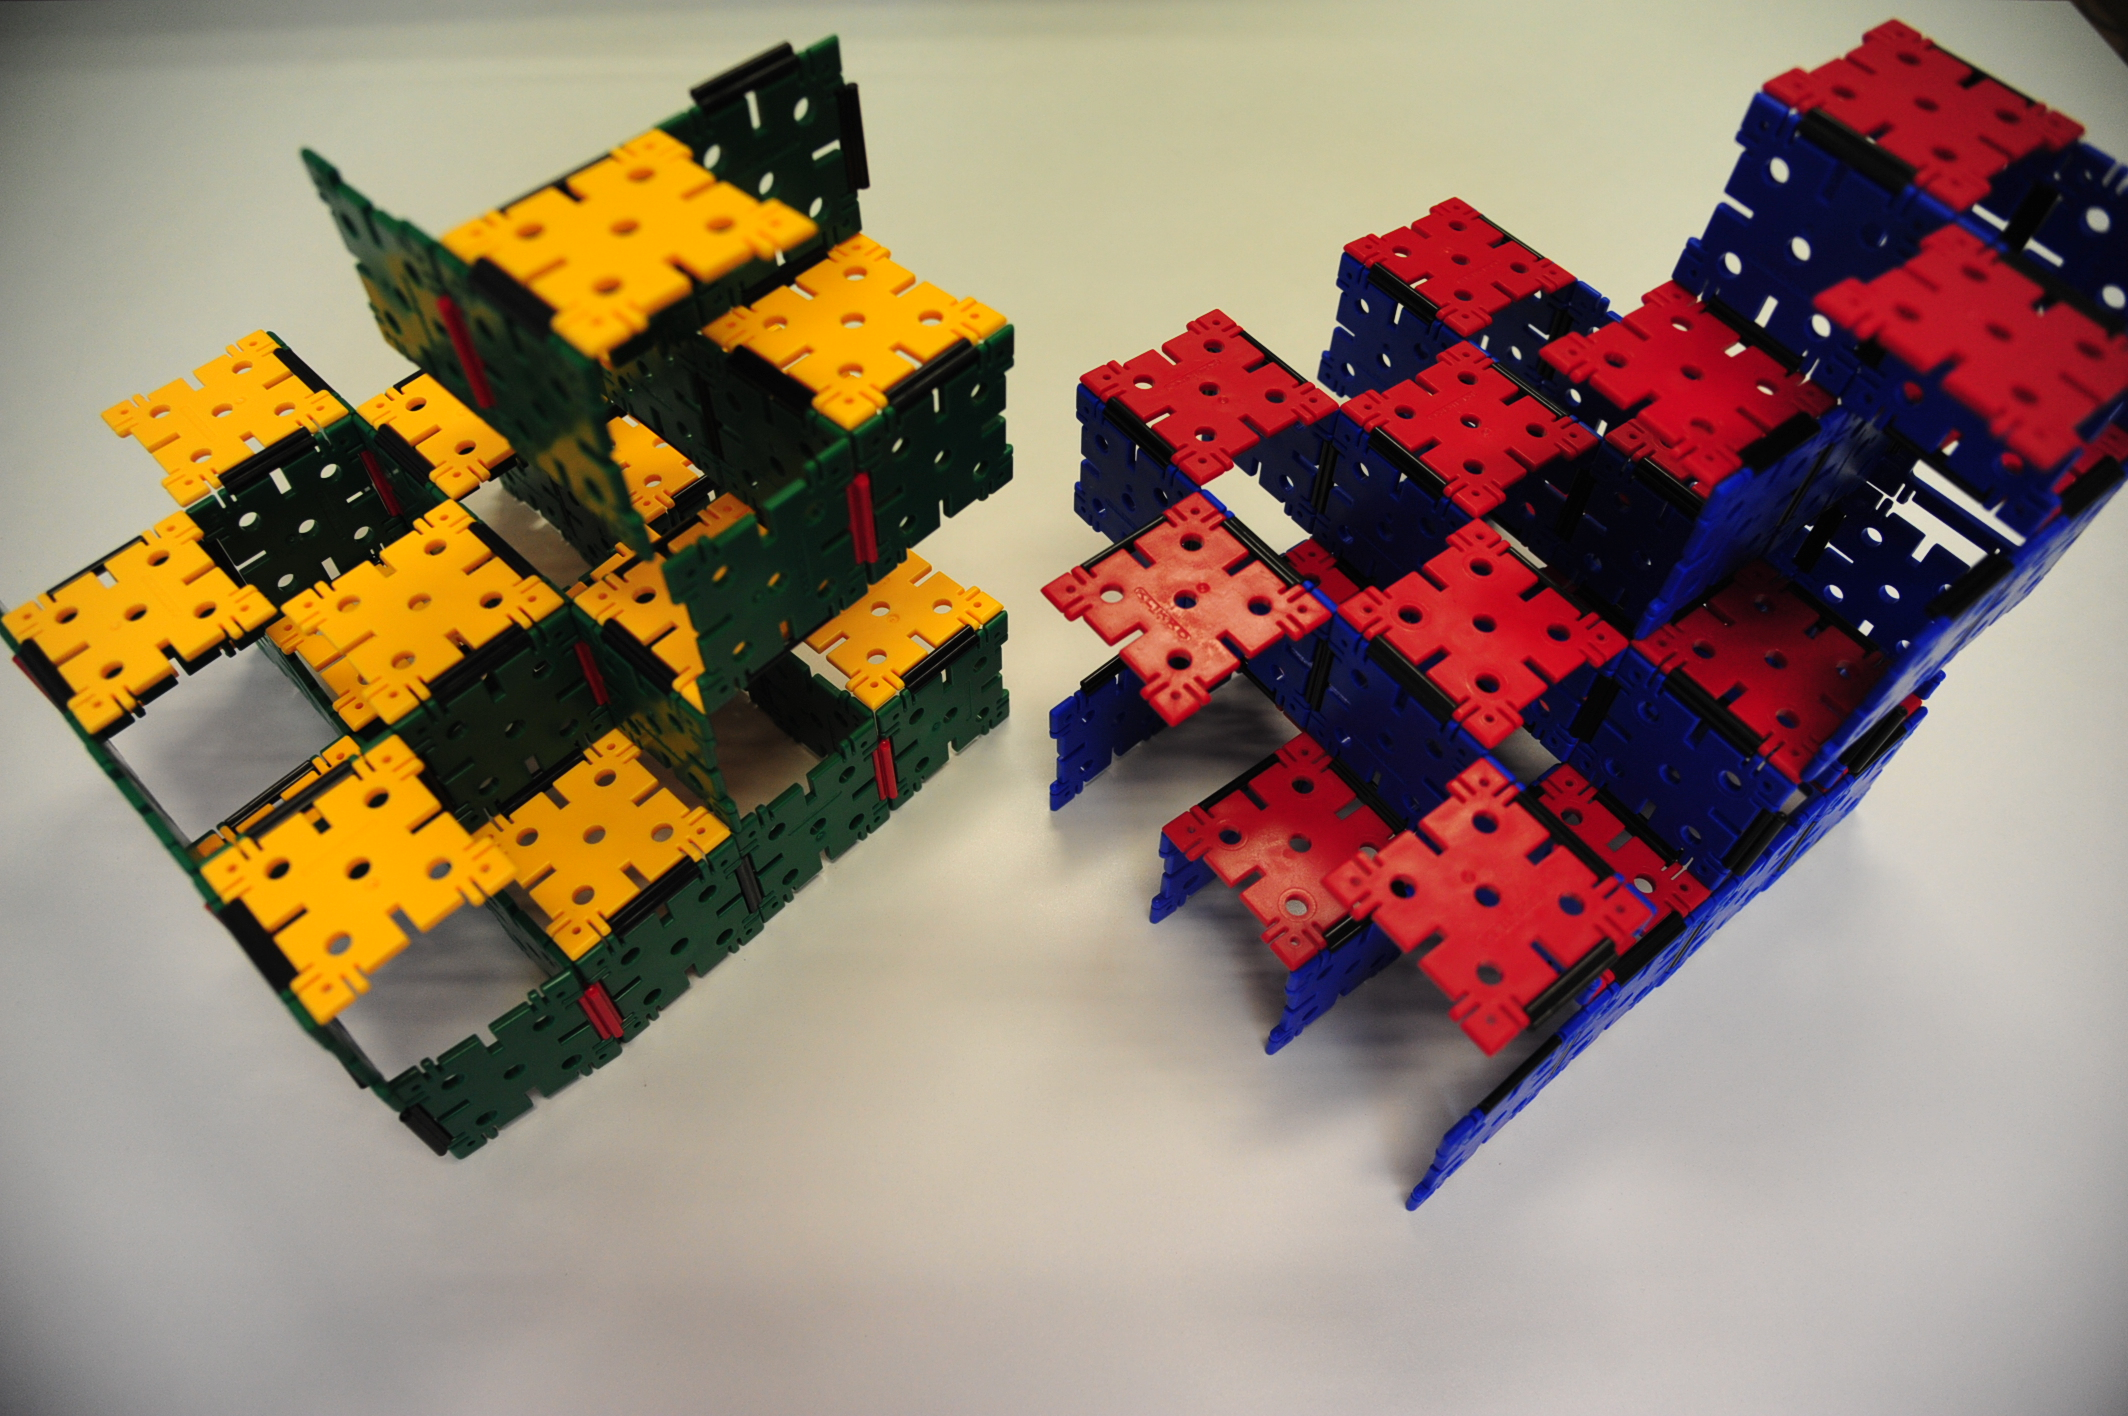
\includegraphics[height=4cm]{toys}
			\end{center}
  \end{frame}
}


% Delete this, if you do not want the table of contents to pop up at
% the beginning of each subsection:

\begin{document}

\begin{frame}
  \titlepage
\end{frame}

\begin{frame}{References}
\begin{itemize}
\item Zhi-Da Song: Princeton University.
\item Chen Fang: Institute of Physics, Beijing.
\begin{center}
	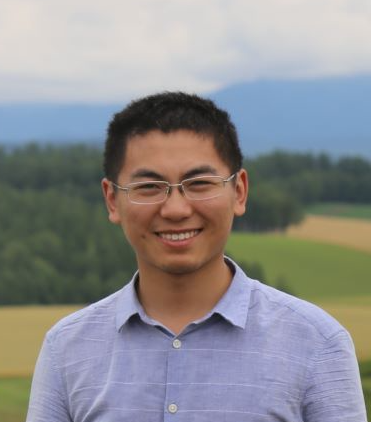
\includegraphics[height=3cm]{../people/zhidasong}
	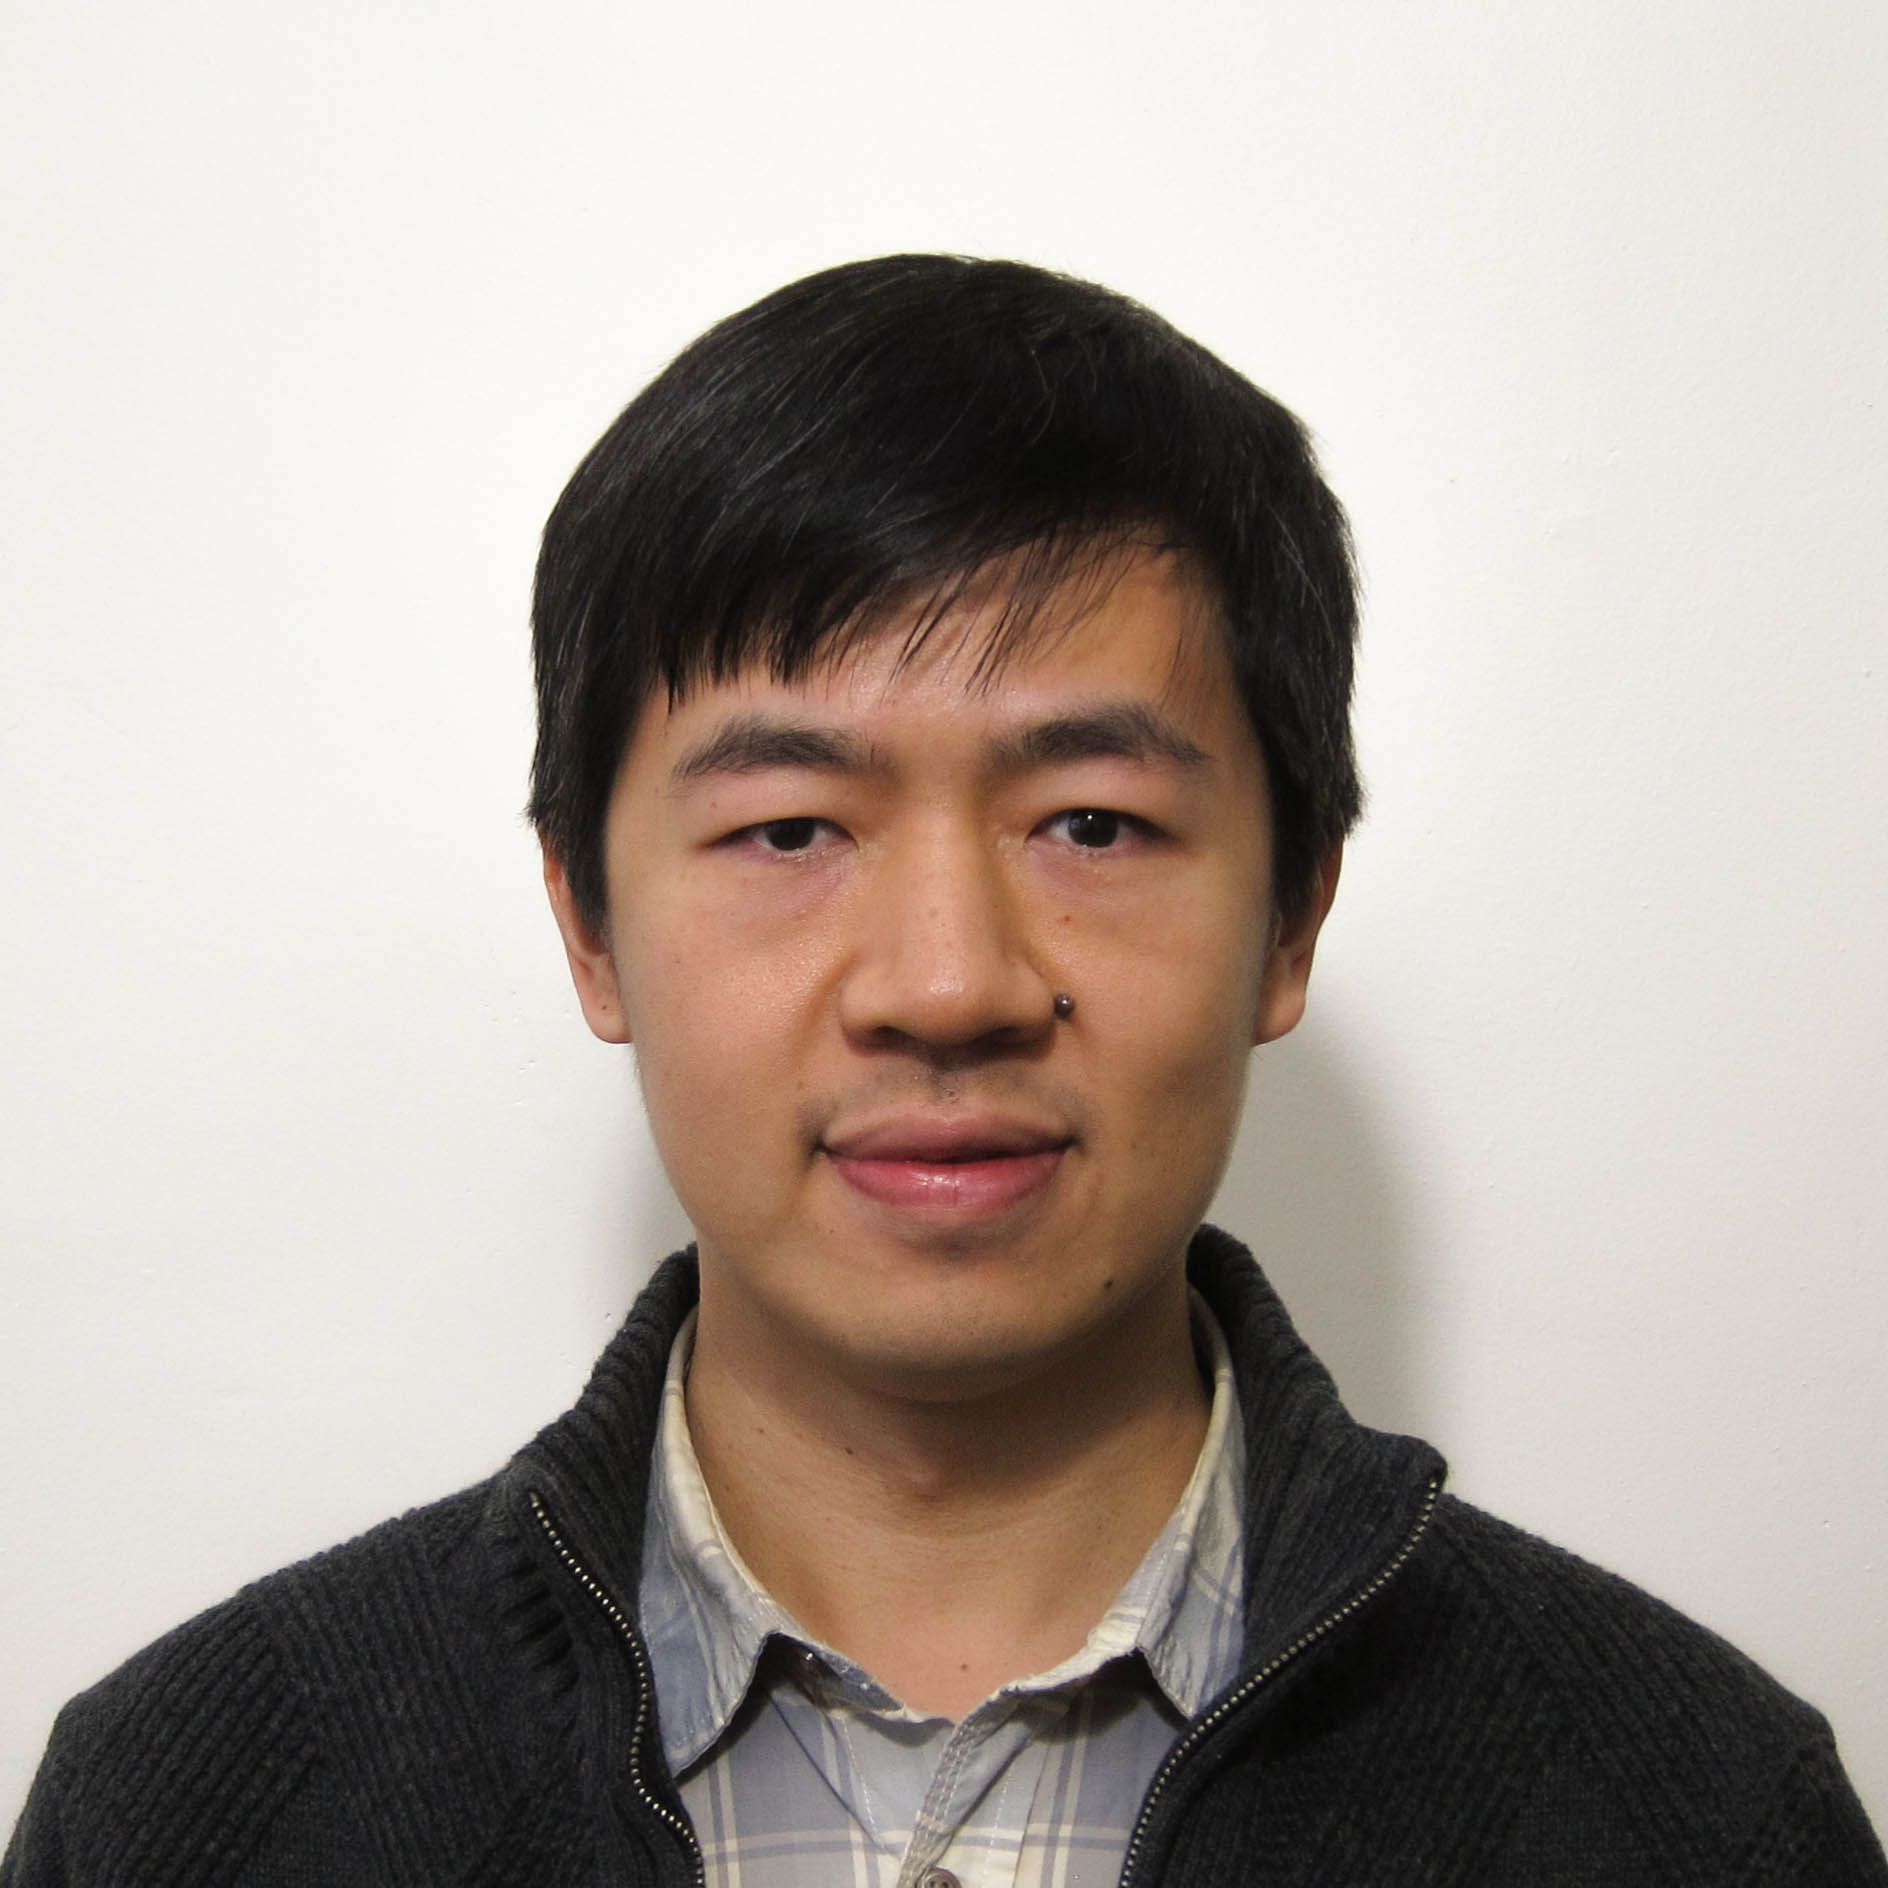
\includegraphics[height=3cm]{../people/chenfang}
\end{center}
\item Zhida Song, Chen Fang and Yang Qi, arXiv:1810.11013
\end{itemize}
\end{frame}

\section{Introduction to Symmetry-Protected Topological (SPT) states}

\begin{frame}
  \frametitle{Symmetry-Protected Topological (SPT) states}
\begin{itemize}
\item SPT: gapped topological phases beyond Landau paradiam.
\item Cannot be smoothly connected to a trivial state without closing gap or breaking symmetry.
\item Symmetry-protected gapless surface states.
\item Free-fermion states: topological insulators, topological superconductors.
\item Bosonic SPTs: Haldane chain, CZX/Levin-Gu state, etc.\\
\emph{Xie Chen, Zheng-Cheng Gu, Zheng-Xin Liu and Xiao-Gang Wen, Science 2012.}
\item Interacting fermionic SPTs.
\end{itemize}
\end{frame}

\begin{frame}
  \frametitle{SPT states of onsite symmetry}
  \begin{itemize}
    \item Classification is given by group cohomology
    \[\Phi^d(G) = H^{d+1}[G, \uone_T].\]
		\item Wave functions are symmetric cochains:
		\[\omega(gg_0,\ldots gg_{d+1})=\rho_T(g)\omega(g_0,\ldots g_{d+1}),\quad
		\omega\in\Psi^d(G) = C^{d+1}[G, \uone_T].\]
		\item Bulk-boundary correspondence:
		\[d\omega = \nu,\quad d:C^d[G, \uone_T]\rightarrow C^{d+1}[G, \uone_T]\]
		\[d\omega(g_0,\ldots,g_{d+1})
		=\sum_i(-1)^i\omega(g_0,\ldots,\hat g_i,\ldots,g_{d+1}).\]
\begin{center}
	\begin{tikzpicture}
	\fill (.5, .5)--(4.5, 0.5)--(5, 1)--(5, 2)--(1, 2)--(0.5, 1.5)--(0.5, 0.5) [mbg!15];
	\node at (2.75, 1.5) {$\nu$};
	\fill (0.5, 0.5)--(4.5, 0.5)--(5, 1)--(1, 1)--(0.5, 0.5) [mbg];
	\node  [text=white] at (2.75, 0.75) {$\omega$};
	\draw (1, 1)--(1, 2) [black!40];
	\draw (0.5, 0.5)--(0.5, 1.5) [black!40];
	\draw (5, 1)--(5, 2) [black!40];
	\end{tikzpicture}
\end{center}
  \item A cohomology group:
\[H^{d+1}[G,\uone_T]=\{d\omega=0\}/\{\omega\simeq\omega+d\mu\}=\frac{\ker d}{\img d}.\]
  \end{itemize}
\end{frame}

\begin{frame}
\frametitle{Space-group SPT}
\begin{itemize}
\item We consider $G\supset SG$.
\item Thorngren and Else (2018): the classification is also given by group cohomology
\[H^{d+1}[G, \uone_{PT}].\]
\item Dimensional reduction: Liang Fu, Michael Hermele et al.\\
\emph{Examples: mirror SPT, weak SPT (translation symmetry).}
\item Patch construction: Zhida Song, Shengjie Huang, Yang Qi, Chen Fang and Michael Hermele, to appear.
\item A more general construction for bosonic SPTs w/ all possible $G$.
\end{itemize}
\begin{center}
\begin{tikzpicture}
\fill [blue!20] (0,0)--(1,1)--(1,3)--(0,2)--(0,0);
\draw (0,0)--(0,2)--(1,3);
\draw (-1.5,0)--(1.5,0)--(1.5,2)--(-1.5,2)--(-1.5,0);
\draw (1.5,0)--(2.5,1)--(2.5,3)--(1.5,2);
\draw (2.5,3)--(-.5,3)--(-1.5,2);
\end{tikzpicture}
\hspace{2em}
\begin{tikzpicture}
\fill [blue!40,opacity=.5] (0,0)--(1,1)--(1,3)--(0,2)--(0,0);
\draw (0,0)--(0,2)--(1,3);
\fill [blue!40,opacity=.5] (.5,0)--(1.5,1)--(1.5,3)--(0.5,2)--(0.5,0);
\draw (.5,0)--(.5,2)--(1.5,3);
\fill [blue!40,opacity=.5] (1,0)--(2,1)--(2,3)--(1,2)--(1,0);
\draw (1,0)--(1,2)--(2,3);
\fill [blue!40,opacity=.5] (-.5,0)--(.5,1)--(.5,3)--(-0.5,2)--(-0.5,0);
\draw (-.5,0)--(-.5,2)--(.5,3);
\fill [blue!40,opacity=.5] (-1,0)--(0,1)--(0,3)--(-1,2)--(-1,0);
\draw (-1,0)--(-1,2)--(0,3);
\draw (-1.5,0)--(1.5,0)--(1.5,2)--(-1.5,2)--(-1.5,0);
\draw (1.5,0)--(2.5,1)--(2.5,3)--(1.5,2);
\draw (2.5,3)--(-.5,3)--(-1.5,2);
\end{tikzpicture}
\end{center}
\end{frame}

\section{Simplified version: 1st and 2nd pages.}
\begin{frame}
	\frametitle{Topological crystalline states are made of building blocks}
	\begin{columns}
		\column{.4\textwidth}
		\begin{center}
			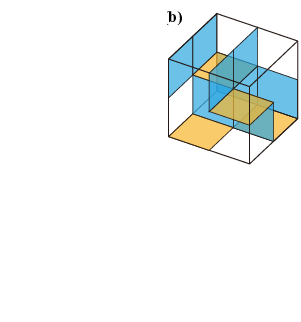
\includegraphics[width=\textwidth]{blocks}
		\end{center}
		\column{.6\textwidth}
		\begin{itemize}
			\item We divide the space into cells compatible with the space-group symmetry.
			\item On a $p$-cell $\sigma$, the SPT state is protected only by $G_\sigma$.
			\[\hat\omega(\sigma)\in \Phi^d(G) = H^{d+1}[G_\sigma,\uone_T].\]
			\item $G_\sigma$ acts as onsite symmetries.
			\item Decorate 3d SPT on 3-cells; 2d SPT on 2-cells; 1d SPT on 1-cells; 0d SPT on 0-cells;
			\item $p$-block states: $E^p_{p,\infty}$.
			\[\text{TCSs} = \bigoplus_p E^p_{p,\infty}.\]
		\end{itemize}
	\end{columns}
\end{frame}

\begin{frame}
	\frametitle{Decomposition of the space}
	We divide the space into finer cells such that
	\begin{enumerate}
		\item A cell $\sigma$ is maped to one single cell $\sigma^\prime$ under $SG$-action.
		\item $G_\sigma$ acts on $\sigma$ as onsite symmetry.
	\end{enumerate}
	\begin{center}
		\begin{tikzpicture}
			\draw (-2, -2)--(-2, 2)--(2, 2)--(2, -2)--(-2, -2);
			\draw [thick] (0, -2)--(0, 2);
			\filldraw (0, 0) circle (1pt) node [right] {$C_2$};
			\node at (0, -1) [right] {$\tau_1$};
			\node at (0, 1) [left] {$\tau_2$};
			\node at (-1, 0) {$\sigma_1$};
			\node at (1, 0) {$\sigma_2$};
		\end{tikzpicture}
	\end{center}
\end{frame}

\begin{frame}
	\frametitle{Symmetric conditions}
	\begin{columns}
		\column{.4\textwidth}
		\begin{tikzpicture}
			\draw (0, 0)--(2, 0)--(2, 2)--(0, 2)--(0, 0);
			\draw (2, 4)--(4, 4)--(4, 6)--(2, 6)--(2, 4);
			\draw [thick,->] (1, 1) node [below] {$\hat\omega(\sigma$)} --
			(3, 5) node [above] {$\hat\omega(\sigma^\prime)$};
			\node at (2, 3) [right] {$g$};
		\end{tikzpicture}
		\column{.6\textwidth}
		\begin{itemize}
			\item If $g:\sigma\rightarrow\sigma^\prime$, then the cochains attached must be ``identical''.
			\item $G_\sigma\neq G_{\sigma'}$, but they are isomorphic:
			\[G_{\sigma'}=gG_\sigma g^{-1}\simeq G_\sigma.\]
			\item This induces another isomorphism between the cohomology classes:
			\[H^{p+1}[G_{\sigma'},\uone_T]\simeq H^{p+1}[G_\sigma,\uone_T]\]
			\item $\hat\omega(\sigma)$ and $\hat\omega(\sigma')$ are related by this isomorphism, which we denote by
			\[\hat\omega(\sigma') = g\cdot \hat\omega(\sigma).\]
			\item Only decorations on symmetry-unrelated cells are independent: finite \# of them.
		\end{itemize}
	\end{columns}
\end{frame}

\begin{frame}
	\frametitle{The 1st page}

	\begin{columns}
		\column{.4\textwidth}
		\begin{center}
			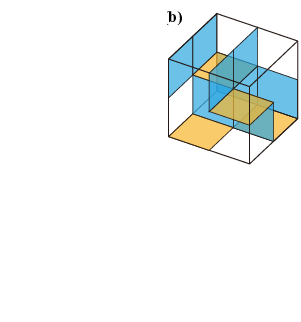
\includegraphics[width=\textwidth]{blocks}
		\end{center}
		\column{.6\textwidth}
		\begin{itemize}
			\item 1st page = a collection of SPTs:
			\[E^p_{p,1} = \bigoplus_{\sigma\in Y_p/G} \Phi^p(G_\sigma),\]
			\[\Phi^p(G_\sigma) = H^{p+1}(G_\sigma, \uone_T).\]
			\item We can generalize this to
			\[E^q_{p,1} = \bigoplus_{\sigma\in Y_p/G} \Phi^q(G_\sigma).\]
		\end{itemize}
	\end{columns}
\end{frame}

\begin{frame}
	\frametitle{No-Open-Edge Conditions}
	\begin{columns}
		\column{.58\textwidth}
		\begin{itemize}
			\item SPT blocks have nontrivial boundary states.
			\item Boundary anomaly must cancel on $(p-1)$-cells.
			\item Naively:
			\[\hat\omega(\sigma_1)
			+\hat\omega(\sigma_2)+\hat\omega(\sigma_3)+\hat\omega(\sigma_4)\]
			\item A subtlety: $\tau$ has more symmetry operations than $\sigma$: $G_\tau \supseteq G_\sigma$
			\item Hence, $\hat\omega(\sigma_i)$ is not $G_\tau$-symmetric.
			\item When $[G_\tau:G_\sigma]>1$: $\tau$ borders $[G_\tau:G_\sigma]$ symmetry-related copies of $\sigma_i$.
			\item $\hat\omega(\sigma_1)
			+\hat\omega(\sigma_2)+\hat\omega(\sigma_3)+\hat\omega(\sigma_4)\in H^{p+1}[G_\tau,\uone_T]$.
		\end{itemize}
		\column{.42\textwidth}
		\begin{tikzpicture}
			\draw (0, 1)--(-1, 1)--(-2, 0)--(2, 0)--(3, 1)--(1, 1);
			\draw [thick] (0, 0)--(1, 1);
			\node at (.5, .5) [above] {$\tau$};
			\draw (1, 1)--(1, 3)--(0, 2)--(0, -2)--(0, -2)--(1, -1)--(1, 0);
			\node at (.5, 1.5) {$\sigma_1$};
			\node at (1.5, .5) {$\sigma_2$};
			\node at (.5, -0.5) {$\sigma_3$};
			\node at (-0.5, .5) {$\sigma_4$};
		\end{tikzpicture}
	\end{columns}
\end{frame}

\begin{frame}
	\frametitle{No-Open-Edge Conditions}
	\begin{columns}
		\column{.58\textwidth}
		\begin{itemize}
			\item We can define a boundary-transfer operation $\partial\omega$:
			\[(\partial\omega)(\tau)=\hat\omega(\sigma_1)
			+\hat\omega(\sigma_2)+\hat\omega(\sigma_3)+\hat\omega(\sigma_4).\]
			\item Cocycle equation: $\partial\omega\simeq0.$
			\item Define $d_1: E^p_{p,1}\rightarrow E^p_{p-1,1}$:
			\[d_1\omega = \partial\omega.\]
			\item First-page no-open-edge condition:
			\[d_1\omega \simeq 0.\]
			\item $E^{p+1}_{p,r}$: anomaly pattern.
		\end{itemize}
		\column{.42\textwidth}
		\begin{tikzpicture}
			\draw (0, 1)--(-1, 1)--(-2, 0)--(2, 0)--(3, 1)--(1, 1);
			\draw [thick] (0, 0)--(1, 1);
			\node at (.5, .5) [above] {$\tau$};
			\draw (1, 1)--(1, 3)--(0, 2)--(0, -2)--(0, -2)--(1, -1)--(1, 0);
			\node at (.5, 1.5) {$\sigma_1$};
			\node at (1.5, .5) {$\sigma_2$};
			\node at (.5, -0.5) {$\sigma_3$};
			\node at (-0.5, .5) {$\sigma_4$};
		\end{tikzpicture}
	\end{columns}
\end{frame}

\begin{frame}
	\frametitle{Bubbling Equivalence}
\begin{columns}
\column{.6\textwidth}
\begin{itemize}
\item Coboundaries: $\omega\simeq0$.
\item A coboundary: attaching the same SPT state to  $\partial \sigma$.
\item The bubbling process can also expressed by $\partial$:
\[\omega = \partial\mu\simeq0.\]
\item We define $d_1:E^p_{p+1, 1}\rightarrow E^p_{p,1}$:
\[d_1\mu = \partial\mu.\]
\item The first-page bubbling equivalence:
\[d_1\mu\simeq0.\]
\item $E^{p+1}_{p,r}$: Bubbling patterns.
\end{itemize}
\column{.4\textwidth}
\begin{animateinline}{5}
        \multiframe{12}{Ra=.8+.1}{
\begin{tikzpicture}
	\draw (-2,-2)--(-2,2)--(2,2)--(2,-2)--(-2,-2);
	%\fill [green!30] (-\Ra,-\Ra)--(-\Ra,\Ra)--(\Ra,\Ra)--(\Ra,-\Ra)--(-\Ra,-\Ra);
\draw [blue,thick] (-\Ra,-\Ra)--(-\Ra,\Ra)--(\Ra,\Ra)--(\Ra,-\Ra)--(-\Ra,-\Ra);
%\node at (0, 0) {$d\nu$};
\node at (\Ra, 0) [left] {$\nu$};
\end{tikzpicture}
}
\end{animateinline}
\end{columns}
\end{frame}

\begin{frame}
\frametitle{2nd page: a homology-group calculation}
\begin{itemize}
\item No-open-edge conditions:
\[d_1\omega\simeq 0.\]
\item Bubbling equivalence:
\[d_1\mu\simeq 0.\]
\item A homology-group calculation:
\[E^p_{p+1,1}\xrightarrow{d_1}E^p_{p,1}\xrightarrow{d_1}E^p_{p-1,1},\]
\[E^p_{p,2}=\frac{\ker d^p_{p+1,1}}{\img d^p_{p,1}}.\]
\end{itemize}
\end{frame}




%\begin{frame}
%	\frametitle{A building block}
%	\begin{columns}
%		\column{.4\textwidth}
%		\begin{center}
%			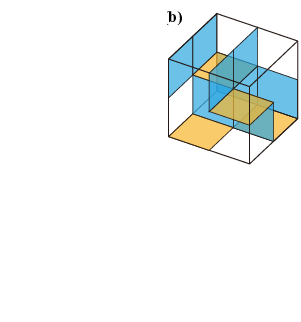
\includegraphics[width=\textwidth]{blocks}
%		\end{center}
%		\column{.6\textwidth}
%		\begin{itemize}
%			\item A building block $\hat\omega$ is a collection of cochains:
%			\[\hat\omega(\sigma) \in C^{p+1}[G_\sigma, \uone_T].\]
%			\item $\hat\omega$ needs to be symmetric under $SG$.
%			\item $\hat\omega$ needs to satisfy the bulk-boundary relation:
%			\[d\hat\omega(\tau) = \sum_{\sigma:\tau\in\partial\sigma}\hat\omega(\sigma).\]
%			\item Need to find when two blocks can be deformed to each other: $\hat\omega\simeq\hat\omega^\prime$.
%		\end{itemize}
%	\end{columns}
%\end{frame}



\section{Full version: higher pages}

\begin{frame}
\frametitle{General construction: a ``perturbative'' approach}
We can classify building blocks according to the leading dimension:
\begin{align*}
E^3_{3,\infty}:\hat\omega_{3+}&= \alert{\hat\omega_3} + \hat\omega_2+ \hat\omega_1+ \hat\omega_0;\\
E^2_{2,\infty}:\hat\omega_{2+}&= \alert{\hat\omega_2}+ \hat\omega_1+ \hat\omega_0;\\
E^1_{1,\infty}:\hat\omega_{1+}&= \alert{\hat\omega_1}+ \hat\omega_0;\\
E^0_{0,\infty}:\hat\omega_{0+}&= \alert{\hat\omega_0};
\end{align*}
\begin{itemize}
\item We only choose a special solution for subleading terms.

\item \alert{Building blocks} / Connectors.
\end{itemize}
\begin{center}
\begin{tikzpicture}[scale=1.5]
\fill [blue!50] (0.1,0.1)--(1,0.1)--(1.4,.5)--(1.4,1.4)--(0.5,1.4)--(.1,1)--(0.1,0.1);
\draw (0,0)--(1,0)--(1,1)--(0,1)--(0,0);
\draw (1,0)--(1.5,.5)--(1.5,1.5)--(1,1);
\draw (1.5,1.5)--(0.5,1.5)--(0,1);
\end{tikzpicture}~~~~
\begin{tikzpicture} [scale=1.5]
\fill [blue!50] (0,0)--(1,0)--(1.5,.5)--(1.5,1.5)--(0.5,1.5)--(0,1)--(0,0);
\draw (0,0)--(1,0)--(1,1)--(0,1)--(0,0);
\draw (1,0)--(1.5,.5)--(1.5,1.5)--(1,1);
\draw (1.5,1.5)--(0.5,1.5)--(0,1);
\draw (0,0)--(.5,.5)--(.5,1.5);
\draw (.5,.5)--(1.5,.5);
\end{tikzpicture}~~~~
\begin{tikzpicture} [scale=1.5]
\draw [thick,blue] (0,0)--(1,0)--(1,1)--(0,1)--(0,0);
\draw [thick,blue](1,0)--(1.5,.5)--(1.5,1.5)--(1,1);
\draw [thick,blue](1.5,1.5)--(0.5,1.5)--(0,1);
\draw [thick,blue](0,0)--(.5,.5)--(.5,1.5);
\draw [thick,blue](.5,.5)--(1.5,.5);
\end{tikzpicture}~~~~
\begin{tikzpicture} [scale=1.5]
\draw (0,0)--(1,0)--(1,1)--(0,1)--(0,0);
\draw (1,0)--(1.5,.5)--(1.5,1.5)--(1,1);
\draw (1.5,1.5)--(0.5,1.5)--(0,1);
\draw (0,0)--(.5,.5)--(.5,1.5);
\draw (.5,.5)--(1.5,.5);
\filldraw [blue] (0,0) circle (2pt);
\filldraw [blue] (1,0) circle (2pt);
\filldraw [blue] (0,1) circle (2pt);
\filldraw [blue] (1,1) circle (2pt);
\filldraw [blue] (0.5,0.5) circle (2pt);
\filldraw [blue] (0.5,1.5) circle (2pt);
\filldraw [blue] (1.5,0.5) circle (2pt);
\filldraw [blue] (1.5,1.5) circle (2pt);
\end{tikzpicture}
\end{center}
\end{frame}

\begin{frame}
	\frametitle{Bulk-Boundary Relations}
	\begin{columns}
		\column{.58\textwidth}
		\begin{itemize}
			\item On the cell $\tau$:
			\[d\hat\omega(\tau) = \hat\omega(\sigma_1)
			+\hat\omega(\sigma_2)+\hat\omega(\sigma_3)+\hat\omega(\sigma_4)\]
			\item $\hat\omega(\sigma_1)
			+\hat\omega(\sigma_2)+\hat\omega(\sigma_3)+\hat\omega(\sigma_4)\in C^{p+1}[G_\tau,\uone_T]$.
			\item Generalize the boundary-transfer operation $\partial\hat\omega$:
			\[(\partial\hat\omega)(\tau)=\hat\omega(\sigma_1)
			+\hat\omega(\sigma_2)+\hat\omega(\sigma_3)+\hat\omega(\sigma_4).\]
			\item Cocycle equation: $d\hat\omega - \partial\hat\omega=0.$
		\end{itemize}
		\column{.42\textwidth}
		\begin{tikzpicture}
			\draw (0, 1)--(-1, 1)--(-2, 0)--(2, 0)--(3, 1)--(1, 1);
			\draw [thick] (0, 0)--(1, 1);
			\node at (.5, .5) [above] {$\tau$};
			\draw (1, 1)--(1, 3)--(0, 2)--(0, -2)--(0, -2)--(1, -1)--(1, 0);
			\node at (.5, 1.5) {$\sigma_1$};
			\node at (1.5, .5) {$\sigma_2$};
			\node at (.5, -0.5) {$\sigma_3$};
			\node at (-0.5, .5) {$\sigma_4$};
		\end{tikzpicture}
	\end{columns}
\end{frame}

\begin{frame}
\frametitle{No-Open-Edge Conditions}
\begin{columns}
\column{.6\textwidth}
\begin{itemize}
\item Consider $\hat\omega_{2+}=\hat\omega_2+\hat\omega_1+\hat\omega_0$.
\item Cocycle condition: $(d+\partial)\hat\omega=0$:
\begin{align*}
d\hat\omega_2&=0;\\
d\hat\omega_1&=\partial\hat\omega_2\simeq0;\\
d\hat\omega_0&=\partial\hat\omega_1\simeq0.
\end{align*}
\end{itemize}
\begin{enumerate}
\item Choose a cocycle for each 2-cell $\sigma$.\\
\emph{0th-page no-open-edge condition.}
\item Check $\partial\hat\omega_2(\tau)\simeq0$ for each 1-cell $\tau$.\\
\emph{1st-page no-open-edge condition.}
\item Choose a cochain $\hat\omega_1$ for each $\tau$.
Check $\partial\hat\omega_1(\lambda)\simeq0$ for each 0-cell $\lambda$.\\
\emph{2nd-page no-open-edge condition.}
\item Choose a cochain $\hat\omega_0$ for each $\lambda$.
\end{enumerate}
\column{.4\textwidth}
\begin{center}
\begin{tikzpicture} [scale=1.5]
\fill [blue!50] (0,0)--(1,0)--(1.5,.5)--(1.5,1.5)--(0.5,1.5)--(0,1)--(0,0);
\draw [thick,white] (0,0)--(1,0)--(1,1)--(0,1)--(0,0);
\draw [thick,white] (1,0)--(1.5,.5)--(1.5,1.5)--(1,1);
\draw [thick,white] (1.5,1.5)--(0.5,1.5)--(0,1);
\draw [thick,white] (0,0)--(.5,.5)--(.5,1.5);
\draw [thick,white](.5,.5)--(1.5,.5);
\fill [white] (0,0) circle (2pt);
\fill [white] (1,0) circle (2pt);
\fill [white] (0,1) circle (2pt);
\fill [white] (1,1) circle (2pt);
\fill [white] (0.5,0.5) circle (2pt);
\fill [white] (1.5,0.5) circle (2pt);
\fill [white] (0.5,1.5) circle (2pt);
\fill [white] (1.5,1.5) circle (2pt);
\end{tikzpicture}\\
\begin{tikzpicture} [scale=1.5]
\fill [blue!50] (0,0)--(1,0)--(1.5,.5)--(1.5,1.5)--(0.5,1.5)--(0,1)--(0,0);
\draw [thick,black!50!green] (0,0)--(1,0)--(1,1)--(0,1)--(0,0);
\draw [thick,thick,black!50!green] (1,0)--(1.5,.5)--(1.5,1.5)--(1,1);
\draw [thick,thick,black!50!green] (1.5,1.5)--(0.5,1.5)--(0,1);
\draw [thick,thick,black!50!green] (0,0)--(.5,.5)--(.5,1.5);
\draw [thick,thick,black!50!green](.5,.5)--(1.5,.5);
\fill [white] (0,0) circle (2pt);
\fill [white] (1,0) circle (2pt);
\fill [white] (0,1) circle (2pt);
\fill [white] (1,1) circle (2pt);
\fill [white] (0.5,0.5) circle (2pt);
\fill [white] (1.5,0.5) circle (2pt);
\fill [white] (0.5,1.5) circle (2pt);
\fill [white] (1.5,1.5) circle (2pt);
\end{tikzpicture}\\
\begin{tikzpicture} [scale=1.5]
\fill [blue!50] (0,0)--(1,0)--(1.5,.5)--(1.5,1.5)--(0.5,1.5)--(0,1)--(0,0);
\draw [thick,black!50!green] (0,0)--(1,0)--(1,1)--(0,1)--(0,0);
\draw [thick,thick,black!50!green] (1,0)--(1.5,.5)--(1.5,1.5)--(1,1);
\draw [thick,thick,black!50!green] (1.5,1.5)--(0.5,1.5)--(0,1);
\draw [thick,thick,black!50!green] (0,0)--(.5,.5)--(.5,1.5);
\draw [thick,thick,black!50!green](.5,.5)--(1.5,.5);
\fill [red] (0,0) circle (2pt);
\fill [red] (1,0) circle (2pt);
\fill [red] (0,1) circle (2pt);
\fill [red] (1,1) circle (2pt);
\fill [red] (0.5,0.5) circle (2pt);
\fill [red] (1.5,0.5) circle (2pt);
\fill [red] (0.5,1.5) circle (2pt);
\fill [red] (1.5,1.5) circle (2pt);
\end{tikzpicture}
\end{center}
\end{columns}
\end{frame}

\begin{frame}
	\frametitle{Bubbling Equivalence}
\begin{columns}
\column{.6\textwidth}
\begin{itemize}
\item Coboundaries: $\hat\omega\sim0$.
\item 1st-page bubbling process: attaching the same SPT state to  $\partial \sigma$.
\item A more general bubbling process:\\
changes both the boundary and the bulk,
\[\hat\omega(\sigma)=d\mu,\quad
\hat\omega(\tau\in\partial\sigma) = \mu.\]
\end{itemize}
\column{.4\textwidth}
\begin{animateinline}{5}
        \multiframe{12}{Ra=.8+.1}{
\begin{tikzpicture}
	\draw (-2,-2)--(-2,2)--(2,2)--(2,-2)--(-2,-2);
	\fill [green!30] (-\Ra,-\Ra)--(-\Ra,\Ra)--(\Ra,\Ra)--(\Ra,-\Ra)--(-\Ra,-\Ra);
\draw [blue,thick] (-\Ra,-\Ra)--(-\Ra,\Ra)--(\Ra,\Ra)--(\Ra,-\Ra)--(-\Ra,-\Ra);
\node at (0, 0) {$d\nu$};
\node at (\Ra, 0) [left] {$\nu$};
\end{tikzpicture}
}
\end{animateinline}
\end{columns}
\end{frame}

\begin{frame}
\frametitle{Bubbling Equivalences}
\begin{itemize}
\item There is a similar algorithm for the bubbling equivalence.
\item Assign 1d SPT states ($d\hat\mu_1=0$) to 3-cells: $\partial\hat\mu_2$ trivializes $\hat\omega_1$ building blocks.
\item If $\partial\hat\mu_2\simeq0$, choose $d\hat\mu_1+\partial\hat\mu_2=0$, then $\partial\hat\mu_1$ trivializes $\hat\omega_0$ building blocks.
\item ......
\end{itemize}
\begin{center}
\begin{animateinline}{5}
        \multiframe{12}{Ra=.4+.05}{
\begin{tikzpicture}
	\draw (-2,-2)--(-2,2)--(2,2)--(2,-2)--(-2,-2);
   \draw (-2,0)--(2,0);
   \draw (0,-2)--(0,2);
	%\fill [green!30] (-\Ra,-\Ra)--(-\Ra,\Ra)--(\Ra,\Ra)--(\Ra,-\Ra)--(-\Ra,-\Ra);
\draw [blue,thick] (-\Ra+1,-\Ra+1)--(-\Ra+1,\Ra+1)--(\Ra+1,\Ra+1)--(\Ra+1,-\Ra+1)--(-\Ra+1,-\Ra+1);
\draw [blue,thick] (-\Ra+1,-\Ra-1)--(-\Ra+1,\Ra-1)--(\Ra+1,\Ra-1)--(\Ra+1,-\Ra-1)--(-\Ra+1,-\Ra-1);
\draw [blue,thick] (-\Ra-1,-\Ra+1)--(-\Ra-1,\Ra+1)--(\Ra-1,\Ra+1)--(\Ra-1,-\Ra+1)--(-\Ra-1,-\Ra+1);
\draw [blue,thick] (-\Ra-1,-\Ra-1)--(-\Ra-1,\Ra-1)--(\Ra-1,\Ra-1)--(\Ra-1,-\Ra-1)--(-\Ra-1,-\Ra-1);
%\node at (0, 0) {$d\nu$};
%\node at (\Ra, 0) [left] {$\nu$};
\end{tikzpicture}
}
\end{animateinline}
~~~~
\begin{animateinline}{5}
        \multiframe{8}{Ra=.8+-.1}{
\begin{tikzpicture}
\draw (-2,0)--(2,0);
\draw (0, -2)--(0, 2);
\draw [blue,thick,double] (-\Ra, 0)--(\Ra,0);
\draw [blue,thick,double] (2-\Ra,0)--(2,0);
\draw [blue,thick,double] (-2+\Ra,0)--(-2,0);
\draw [blue,thick,double] (0, -\Ra)--(0, \Ra);
\draw [blue,thick,double] (0, 2-\Ra)--(0, 2);
\draw [blue,thick,double] (0, -2+\Ra)--(0, -2);
\fill [red] (-\Ra,0) circle (2pt);
\fill [red] (\Ra,0) circle (2pt);
\fill [red] (0,-\Ra) circle (2pt);
\fill [red] (0,\Ra) circle (2pt);
\fill [red] (2-\Ra,0) circle (2pt);
\fill [red] (-2+\Ra,0) circle (2pt);
\fill [red] (0,2-\Ra) circle (2pt);
\fill [red] (0,-2+\Ra) circle (2pt);
\end{tikzpicture}
}
\end{animateinline}
\end{center}
\end{frame}

\begin{frame}
\frametitle{A spectral sequence}
We compute in the following sequence:
\begin{enumerate}
\item 0st-page no-open-edge condition + 0st-page bubbling equivalence.
\[E^p_{p,1}=\frac{\ker d_0}{\img d_0}.\]
\item 1st-page no-open-edge condition + 0st-page bubbling equivalence.
\[E^p_{p,2}=\frac{\ker d_1}{\img d_1}.\]
\item 2nd-page no-open-edge condition + 0st-page bubbling equivalence.
\[E^p_{p,3}=\frac{\ker d_2}{\img d_2}.\]
\end{enumerate}

\[E^p_{p,1}\supseteq E^p_{p,2}\supseteq E^p_{p,3}\supseteq\cdots=E^p_{p,\infty}.\]
\end{frame}

\begin{frame}
\frametitle{First Page}
\begin{center}
\begin{tikzpicture}
\draw (0,0)--(4,0)--(4,2)--(0,2)--(0,0);
\node at (2,1) {$\hat\omega(\sigma)$};
\end{tikzpicture}
\end{center}
\begin{itemize}
\item The first page concerns only the building blocks.
\item $d\hat\omega(\sigma)=0$.
\item $d\hat\mu(\sigma)\sim0$.
\item Define $d_0=d$.
\end{itemize}
\[E^p_{p,1}=\frac{\ker d_0}{\img d_0}
=\bigoplus_{\sigma\in Y_p/G}H^p(G_\sigma, U(1)_T).\]
\end{frame}

\begin{frame}
\frametitle{Second Page}
\begin{center}
		\begin{tikzpicture}[scale=.6]
			\draw (0, 1)--(-1, 1)--(-2, 0)--(2, 0)--(3, 1)--(1, 1);
			\draw [thick] (0, 0)--(1, 1);
			\node at (.5, .5) [above] {$\tau$};
			\draw (1, 1)--(1, 3)--(0, 2)--(0, -2)--(0, -2)--(1, -1)--(1, 0);
			\node at (.5, 1.5) {$\sigma_1$};
			\node at (1.5, .5) {$\sigma_2$};
			\node at (.5, -0.5) {$\sigma_3$};
			\node at (-0.5, .5) {$\sigma_4$};
		\end{tikzpicture}
~~~~
\begin{animateinline}{5}
        \multiframe{12}{Ra=.4+.05}{
\begin{tikzpicture}[scale=.6]
	\draw (-2,-2)--(-2,2)--(2,2)--(2,-2)--(-2,-2);
   \draw (-2,0)--(2,0);
   \draw (0,-2)--(0,2);
	%\fill [green!30] (-\Ra,-\Ra)--(-\Ra,\Ra)--(\Ra,\Ra)--(\Ra,-\Ra)--(-\Ra,-\Ra);
\draw [blue,thick] (-\Ra+1,-\Ra+1)--(-\Ra+1,\Ra+1)--(\Ra+1,\Ra+1)--(\Ra+1,-\Ra+1)--(-\Ra+1,-\Ra+1);
\draw [blue,thick] (-\Ra+1,-\Ra-1)--(-\Ra+1,\Ra-1)--(\Ra+1,\Ra-1)--(\Ra+1,-\Ra-1)--(-\Ra+1,-\Ra-1);
\draw [blue,thick] (-\Ra-1,-\Ra+1)--(-\Ra-1,\Ra+1)--(\Ra-1,\Ra+1)--(\Ra-1,-\Ra+1)--(-\Ra-1,-\Ra+1);
\draw [blue,thick] (-\Ra-1,-\Ra-1)--(-\Ra-1,\Ra-1)--(\Ra-1,\Ra-1)--(\Ra-1,-\Ra-1)--(-\Ra-1,-\Ra-1);
%\node at (0, 0) {$d\nu$};
%\node at (\Ra, 0) [left] {$\nu$};
\end{tikzpicture}
}
\end{animateinline}
\end{center}
\begin{itemize}
\item No-open-edge condition: $\partial\hat\omega_2\sim0$.
\item Bubbling equivalence: $\hat\omega_2\rightarrow\hat\omega_2+\partial\hat\mu_3$.
\item Define $d_1=\partial:E^q_{p,1}\rightarrow E^q_{p-1,1}$.
\end{itemize}
\[E^p_{p,2}=\frac{\ker d_1}{\img d_1}.\]
\end{frame}

\begin{frame}
\frametitle{Third Page}
\begin{center}
\begin{tikzpicture} [scale=1.5]
\fill [blue!50] (0,0)--(1,0)--(1.5,.5)--(1.5,1.5)--(0.5,1.5)--(0,1)--(0,0);
\draw [thick,black!50!green] (0,0)--(1,0)--(1,1)--(0,1)--(0,0);
\draw [thick,thick,black!50!green] (1,0)--(1.5,.5)--(1.5,1.5)--(1,1);
\draw [thick,thick,black!50!green] (1.5,1.5)--(0.5,1.5)--(0,1);
\draw [thick,thick,black!50!green] (0,0)--(.5,.5)--(.5,1.5);
\draw [thick,thick,black!50!green](.5,.5)--(1.5,.5);
\fill [red] (0,0) circle (2pt);
\fill [red] (1,0) circle (2pt);
\fill [red] (0,1) circle (2pt);
\fill [red] (1,1) circle (2pt);
\fill [red] (0.5,0.5) circle (2pt);
\fill [red] (1.5,0.5) circle (2pt);
\fill [red] (0.5,1.5) circle (2pt);
\fill [red] (1.5,1.5) circle (2pt);
\end{tikzpicture}
~~~~
\begin{animateinline}{5}
        \multiframe{12}{Ra=.4+.05}{
\begin{tikzpicture}[scale=.6]
	\draw (-2,-2)--(-2,2)--(2,2)--(2,-2)--(-2,-2);
   \draw (-2,0)--(2,0);
   \draw (0,-2)--(0,2);
	%\fill [green!30] (-\Ra,-\Ra)--(-\Ra,\Ra)--(\Ra,\Ra)--(\Ra,-\Ra)--(-\Ra,-\Ra);
\draw [blue,thick] (-\Ra+1,-\Ra+1)--(-\Ra+1,\Ra+1)--(\Ra+1,\Ra+1)--(\Ra+1,-\Ra+1)--(-\Ra+1,-\Ra+1);
\draw [blue,thick] (-\Ra+1,-\Ra-1)--(-\Ra+1,\Ra-1)--(\Ra+1,\Ra-1)--(\Ra+1,-\Ra-1)--(-\Ra+1,-\Ra-1);
\draw [blue,thick] (-\Ra-1,-\Ra+1)--(-\Ra-1,\Ra+1)--(\Ra-1,\Ra+1)--(\Ra-1,-\Ra+1)--(-\Ra-1,-\Ra+1);
\draw [blue,thick] (-\Ra-1,-\Ra-1)--(-\Ra-1,\Ra-1)--(\Ra-1,\Ra-1)--(\Ra-1,-\Ra-1)--(-\Ra-1,-\Ra-1);
%\node at (0, 0) {$d\nu$};
%\node at (\Ra, 0) [left] {$\nu$};
\end{tikzpicture}
}
\end{animateinline}
~~~~
\begin{animateinline}{5}
        \multiframe{8}{Ra=.8+-.1}{
\begin{tikzpicture}[scale=.6]
\draw (-2,0)--(2,0);
\draw (0, -2)--(0, 2);
\draw [blue,thick,double] (-\Ra, 0)--(\Ra,0);
\draw [blue,thick,double] (2-\Ra,0)--(2,0);
\draw [blue,thick,double] (-2+\Ra,0)--(-2,0);
\draw [blue,thick,double] (0, -\Ra)--(0, \Ra);
\draw [blue,thick,double] (0, 2-\Ra)--(0, 2);
\draw [blue,thick,double] (0, -2+\Ra)--(0, -2);
\fill [red] (-\Ra,0) circle (2pt);
\fill [red] (\Ra,0) circle (2pt);
\fill [red] (0,-\Ra) circle (2pt);
\fill [red] (0,\Ra) circle (2pt);
\fill [red] (2-\Ra,0) circle (2pt);
\fill [red] (-2+\Ra,0) circle (2pt);
\fill [red] (0,2-\Ra) circle (2pt);
\fill [red] (0,-2+\Ra) circle (2pt);
\end{tikzpicture}
}
\end{animateinline}
\end{center}
\begin{itemize}
\item Define $d_2:E^q_{p,2}\rightarrow E^{q-1}_{p-2,2}$:
\begin{enumerate}
\item Start from $\hat\omega_p$.
\item Find the connectors $\hat\omega_{p-1}$, s.t. $d\hat\omega_{p-1}=\partial\hat\omega_p$.
\item Compute $d_2\hat\omega_p=\partial\hat\omega_{p-1}$.
\end{enumerate}
\item No-open-edge condition: $d_2\hat\omega_p\sim0$.
\item Bubbling equivalence: $\hat\omega_p\rightarrow\hat\omega_p+d_2\hat\omega_{p+2}$.
\end{itemize}
\[E^p_{p,3}=\frac{\ker d_2}{\img d_2}.\]
\end{frame}

\begin{frame}
\frametitle{Final step: the group extension problem}
\begin{itemize}
\item Assume we have computed the classification $\Omega_{p+}=\{\hat\omega_{p+}\}$.
\item The classification may not be simply $\Omega_{3+}\oplus\Omega_{2+}\oplus \Omega_{1+} \oplus \Omega_{0+} $.
\item Example: consider two $2+$ blocks
\begin{align*}
\hat\omega_{2+}=\hat\omega_2+\hat\omega_1+\hat\omega_0;\\
\hat\omega_{2+}'=\hat\omega_2'+\hat\omega_1'+\hat\omega_0'.
\end{align*}
\item If the sum is trivial in $\Omega_{2+}$: $\hat\omega_2+\hat\omega_2^\prime\simeq0$.
\item The subleading term may be nontrivial: $\hat\omega_1+\hat\omega_1'$. So this is a nontrivial term in $\Omega_{1+}$.
\item Need to compute the group-extension problem: can be done if we know all $\hat\omega_i$ explicitly.
\end{itemize}
\end{frame}

\begin{frame}
\frametitle{Some simplifications}
\begin{itemize}
\item If $G = SG\times G_0$.
\item If we ignore $\Omega_0$: not treating the atomic insulators as nontrivial SPTs.
\item Only need to check things to the first order:
\begin{enumerate}
\item $\Omega_{2+}$: assign 2d SPTs to 2-cells, and check-anomaly vanishing on 1-cells. Coboundaries are assigning 2d SPTs to 3-cells.
\item $\Omega_{1+}$: assign 1d SPTs to 1-cells, and check-anomaly vanishing on 0-cells. Coboundaries are assigning 1d SPTs to 2-cells.
\end{enumerate}
\item Trivial group extension: $\Omega_{2+}\oplus\Omega_{1+}$.
\end{itemize}
\end{frame}

\begin{frame}
\frametitle{An example of a nontrivial building block}
Consider $G=SG\times\mathbb Z_2$, $SG=P4_22_12$ (\#94 space group).
\begin{center}
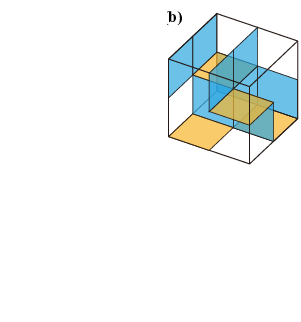
\includegraphics[height=4cm]{blocks}
\end{center}
Each colored 2-cell is decorated with a Levin-Gu or CZX state protected by the onsite $\mathbb Z_2$.

\emph{\small Adapted from Z Song, Y Huang, YQ, C Fang and M Hermele, to appear.}
\end{frame}

\begin{frame}
\frametitle{An example of 2nd order computation}
\emph{\small Adapted from Xu Yang, Shenghan Jiang, Ashvin Vishwanath and Ying Ran, arXiv:1705.09298.}
\begin{itemize}
	\item Consider a magnetic translation symmetry $T_xT_yT_x^{-1}T_y^{-1} = X$, and $G_0=\mathbb Z_2^X\times\mathbb Z_2^T$.
	\item $H^3[G_0,\uone_T]=\mathbb Z_2\oplus\mathbb Z_2$: the one protected by both $\mathbb Z_2^X$ and $\mathbb Z_2^T$ is \alert{not compatible} with the magnetic translation symmetry.
	\item Try to decorate $\omega\in H^3[G_0,\uone_T]$ to all 2-cells: the 1-cells can be gapped out, but the 0-cells \alert{cannot}.
	\item There must be a $T^2=-1$ Kramers doublet at each 0-cell.
\end{itemize}
\begin{center}
\begin{tikzpicture}
\draw (-1.2,0)--(1.2,0);
\draw (-1.2,1)--(1.2,1);
\draw (-1.2,-1)--(1.2,-1);
\draw (-1,-1.2)--(-1,1.2);
\draw (0,-1.2)--(0,1.2);
\draw (1,-1.2)--(1,1.2);
\fill [red] (-1,-1) circle (2pt);
\fill [red] (-1,0) circle (2pt);
\fill [red] (-1,1) circle (2pt);
\fill [red] (0,-1) circle (2pt);
\fill [red] (0,0) circle (2pt);
\fill [red] (0,1) circle (2pt);
\fill [red] (1,-1) circle (2pt);
\fill [red] (1,0) circle (2pt);
\fill [red] (1,1) circle (2pt);
\end{tikzpicture}
\end{center}
\end{frame}

%\section{Mathematical details}
\section{Conclusion}

\begin{frame}
\frametitle{Some mathematical claims}
\begin{itemize}
\item Equivariant group cohomology:
\[H^{d+1}[G, \uone_{PT}]]=H^{d+1}_G[X, \uone_{PT}].\]
Here $X$ is a (non-free) $G$-complex. See Thorngren and Else (2018).
\item There is a spectral sequence:
\[E_1^{pq}=\bigoplus_{\sigma\in X_p/G}H^q[G_\sigma,\uone_T]\Rightarrow
H^{p+q}_G[X,\uone_{PT}].\]
See Brown's book, Chapter VII.
\item The topological space we used is the dual of $X$.
\end{itemize}
\begin{center}
	
\includegraphics[height=2cm]{brown_book}
	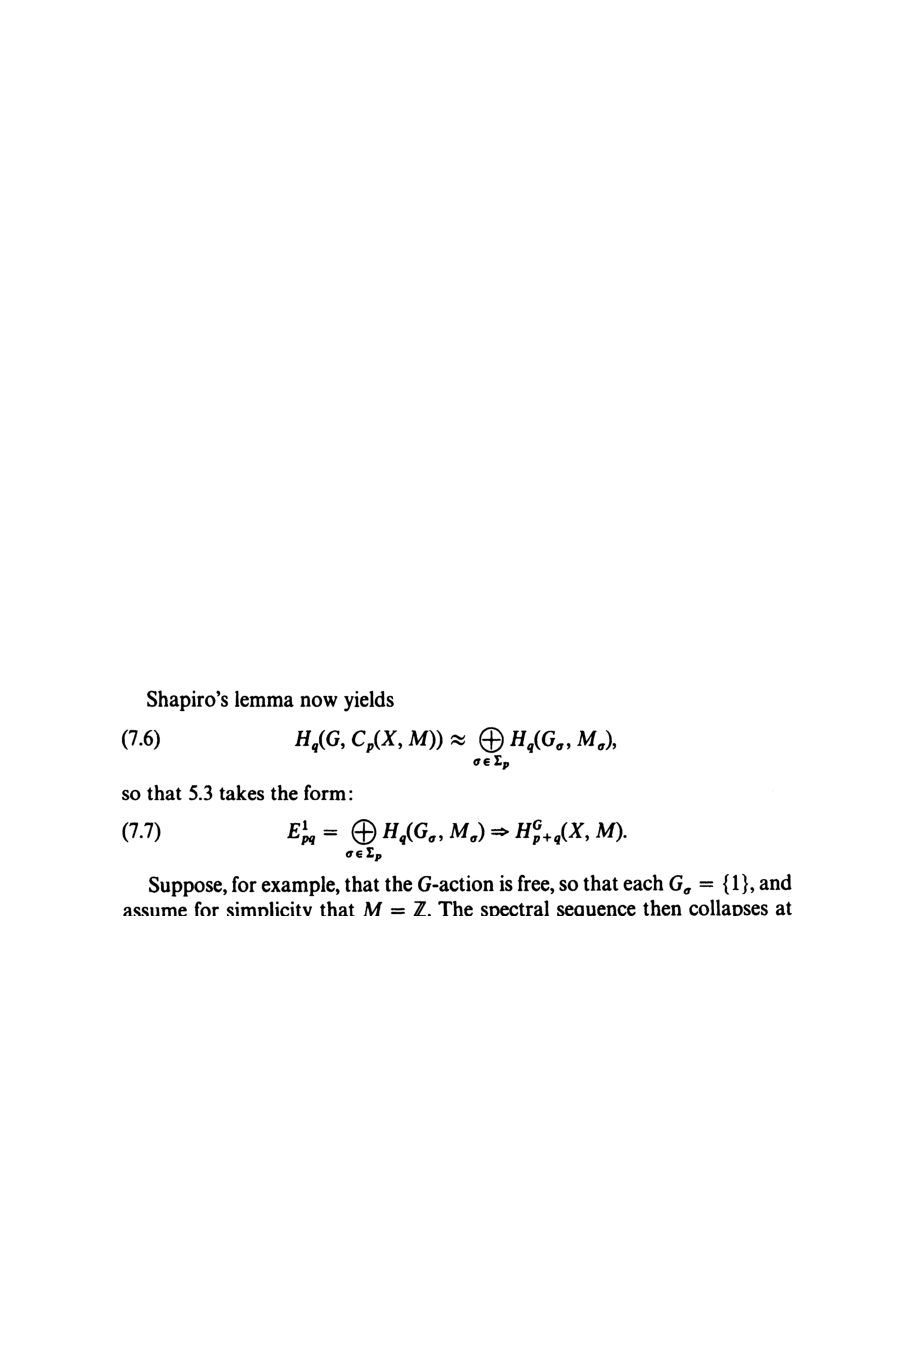
\includegraphics[height=2cm]{brown_ss}
\end{center}
\end{frame}

\begin{frame}
\frametitle{Summary}
\begin{itemize}
\item We develop a way to sysmetically construct space-group SPTs.
\item Check cocycle conditions and coboundary equivalences order-by-order.
\item For $G=SG\times G_0$, first order is enought.
\item Examples beyond simple layered construction.
\item Examples where first-order calculation is not enough.
\end{itemize}
\end{frame}

\begin{frame}
\frametitle{Outlooks}
\begin{itemize}
\item Outlook: cut-and-glue other things:
\begin{enumerate}
\item Bosonic SPTs beyond group cohomology (E8 decorations).
\item Fermionic space-group SPTs.
\item 2D space-group SETs.
\end{enumerate}
\item A way to simplify computations for arbitrary symmetry groups.\\
See M Cheng and C Wang, arXiv:1810.12308.
\item Another work about spectral sequence: Ken Shiozaki, Masatoshi Sato and Kiyonori Gomi, arXiv:1802.06694 (momentum-space analysis).
\item An independent work: Else and Thorngren, arXiv:1810.10539.
\item Related work: K. Shiozaki, C. Zhaoxi Xiong, and K. Gomi,
arXiv:1810.00801.
\end{itemize}
\end{frame}

\end{document}
